\section{Harmonogram pracy maszyn i urządzeń}

\begin{figure}[h]
	\centering
	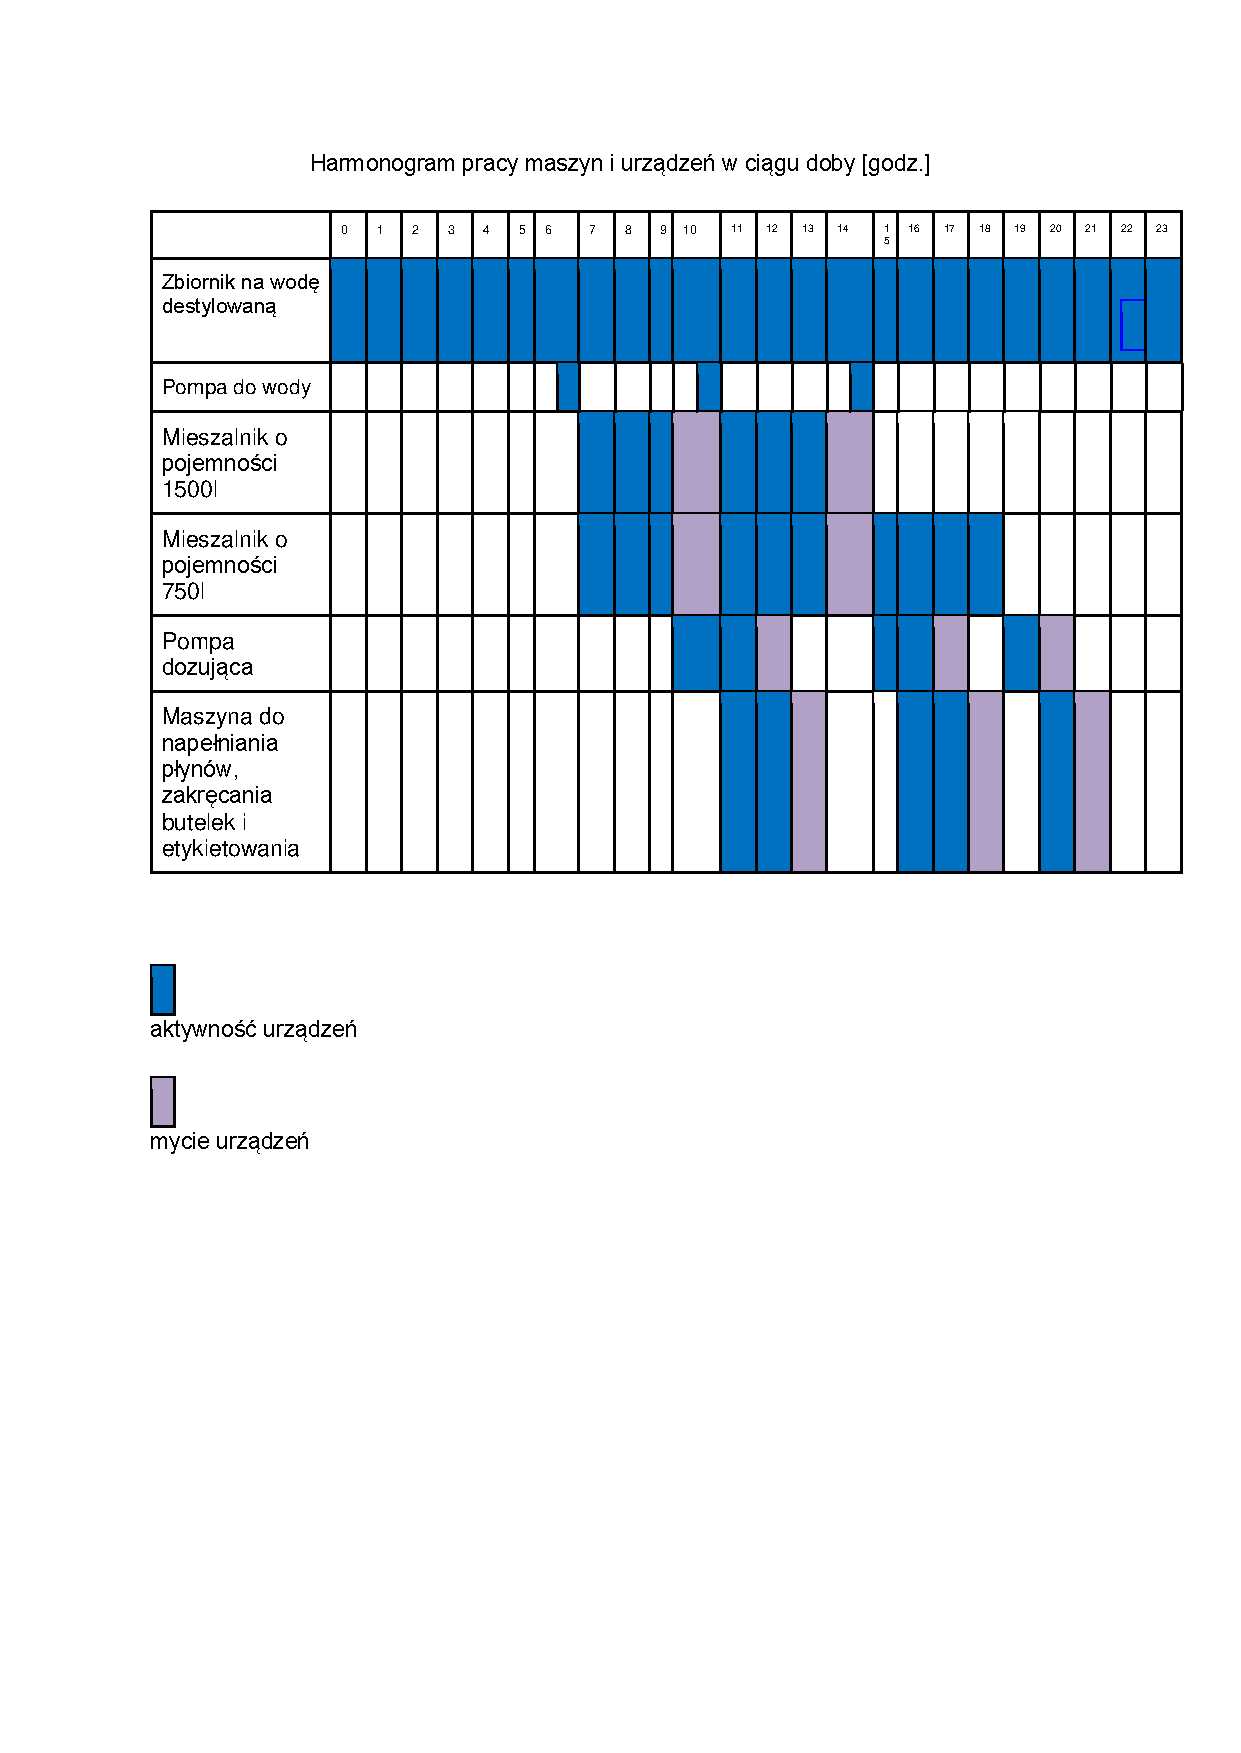
\includegraphics[width=0.9\textwidth]{./sec15/harmonogram_maszyny.pdf}
\end{figure}

%Zakład otwierany będzie o 6.00, do 6.30 będzie wszystko uruchamiane i przygotowywane do produkcji, od 6:30 do 7.00 będzie pompowana woda i dodawane składniki do mieszalnika.\vspace{\baselineskip}
%
%Pompa do wody (\textsf{Speroni CAM80}) – 1h dziennie (ok 25 minut na szampon ziołowy, 15 minut na szampon peelingujący, ok 8 minut na odżywkę proteinową, ok 5 minut na odżywkę emolientową, ok 7 minut na odżywkę humektantową)\vspace{\baselineskip}
%
%Mieszalnik (\textsf{ZRJ - 1500}):
%\begin{itemize}
	%\item praca od 7.00 do 9.30 przy produkcji szamponu ziołowego
	%\item praca od 11.30 do 14.00 przy produkcji szamponu peelingującego
	%\item łącznie :5 h dziennie przez 5 dni w tygodniu
%\end{itemize}\vspace{\baselineskip}
%
%Mieszalnik (\textsf{ZRJ – 750}):
%\begin{itemize}
	%\item praca od 7.00 do 9.30 przy produkcji odżywki proteinowej
	%\item praca od 11.30 do 14.00 przy produkcji odżywki emolientowej
	%\item praca od 16.00 do 18.30 przy produkcji odżywki humektantowej
	%\item łącznie 7,5 h dziennie przez 5 dni w tygodniu
%\end{itemize}\vspace{\baselineskip}
%
%Próbki sprawdzane w laboratorium:
%\begin{itemize}
%\item od 9.30 do 10.30 szampon ziołowy
%\item od 14.00 do 15.00 szampon peelingujący
%\item od 9.30 do 10.30 odżywka proteinowa
%\item od 14.00 do 15.00 odżywka emolientowa
%\item od 18.30 do 19.30 odżywka humektantowa
%\end{itemize}\vspace{\baselineskip}
%
%Pompa dozująca (\textsf{EURALCA}):
%\begin{itemize}
%\item praca od 10.30 do 12.30 przy produkcji szamponu ziołowego
%\item praca od 15.00 do 17.00 przy produkcji szamponu peelingującego
%\item praca od 10.30 do 11.30 przy produkcji odżywki proteinowej
%\item praca od 15.00 do 16.00 przy produkcji odżywki emolientowej
%\item praca od 19.30 do 20.30 przy produkcji odżywki humektantowej
%\end{itemize}
%Łącznie 7h dziennie przez 5 dni w tygodniu ( po 2h na każdy szampon, po 1h na każdą odżywkę)\vspace{\baselineskip}
%
%Maszyna do napełniania płynów, zakręcania butelek i etykietowania:
%\begin{itemize}
%\item praca od 11.00 do 13.00 przy produkcji szamponu ziołowego
%\item praca od 15.30 do 17.30 przy produkcji szamponu peelingującego
%\item praca od 11.00 do 12.00 przy produkcji odżywki proteinowej
%\item praca od 15.30 do 16.30 przy produkcji odżywki emolientowej
%\item praca od 20.00 do 21.00 przy produkcji odżywki humektantowej
%\end{itemize}\vspace{\baselineskip}
%
%(Napełniarka rzędowa AT – L16 typ NPACK):
%
%Łącznie 7h dziennie przez 5 dni w tygodniu ( 2h na każdy szampon, 1h na każdą odżywkę)\vspace{\baselineskip}
%
%(Obrotowa maszyna wlotowa NPACK – J):
%
%Łącznie 4h 15 minut dziennie przez 5 dni w tygodniu  (1h na każdy szampon, 45 minut na każdą odżywkę)\vspace{\baselineskip}
%
%(Maszyna do etykietowania butelek NPACK -TB – YP):
%
%Łcznie 4h 15 minut dziennie przez 5 dni w tygodniu  (1h na każdy szampon, 45 minut na każdą odżywkę)\vspace{\baselineskip}
%
